\documentclass[letterpaper,12pt]{article}
\usepackage{ifthen}
\usepackage{times}
\usepackage{amsmath}
\usepackage{amssymb}
\usepackage{helvet}
\usepackage{courier}
\usepackage{fancyheadings}
\usepackage{hyperref}
\usepackage{comment}
\pagestyle{fancy}
\usepackage{pmc}
\usepackage{graphicx}
\setlength\textwidth{6.5in}
\setlength\textheight{8.5in}

%%%%%%%%%%%%%%%%%%%%%%%%%%%%%%%%%%%%%%%%%%%%%%%%%%%%%%%%%%%%%%%%%%%%%%%%%%%%%%%%%%
% Special for e-unibus doc commands

\newcommand{\ForLater}{
\begin{center}
{\bf NOT FOR CURRENT VERSION}
\end{center}
}
\newcommand{\TBC}{\framebox{\textbf{TO BE COMPLETED}}}
\newcommand{\DISCUSS}{\Ovalbox {\bf \textcolor{red}{FOR DISCUSSION}}}
\newcommand{\Input}{\framebox{\textsf{in}}}
\newcommand{\Output}{\framebox{\textsf{out}}}
\newcommand{\debug}[1]{\textbf{debug start} #1 \textbf{debug finish}}
\newcommand{\inx}[1]{\emph{#1}}
\newtheorem{notation}{Notation}
\newtheorem{definition}{Definition}
\newtheorem{problem_statement}{Problem Statement}
\newtheorem{invariant}{Invariant}
\newtheorem{assumption}{Assumption}
\newtheorem{resource_string}{Resource String}
\newtheorem{testcase}{Test Case}
\newtheorem{note}{Note}
\newtheorem{specification}{Specification}
\newtheorem{caution}{Caution}
\newtheorem{prereq}{Pre-requisite}
\newtheorem{action}{Action}
\newtheorem{query}{Query}
\newcommand{\beq}{\begin{equation}} %% new, no conflict
\newcommand{\eeq}{\end{equation}} %% new, no conflict
\newcommand{\be}{\begin{enumerate}}
\newcommand{\ee}{\end{enumerate}}
\newcommand{\bi}{\begin{itemize}}
\newcommand{\ei}{\end{itemize}}
\newcommand{\bv}{\begin{verbatim}}
\newcommand{\ev}{\end{verbatim}}
\newcommand{\bd}{\begin{description}}
\newcommand{\ed}{\end{description}}
\newcommand{\bpre}{\begin{prereq}}
\newcommand{\epre}{\end{prereq}}
\newcommand{\bact}{\begin{action}}
\newcommand{\eact}{\end{action}}
\newcommand{\bs}{\begin{specification}}
\newcommand{\es}{\end{specification}}
\newcommand{\btc}{\begin{testcase}}
\newcommand{\etc}{\end{testcase}}
\newcommand{\bc}{\begin{caution}}
\newcommand{\ec}{\end{caution}}
\newcommand{\la}{\leftarrow}
\newcommand{\IpArgs}{\subsection{Input Arguments}}
\newcommand{\PreReqs}{\subsection{Pre-requisities}}
\newcommand{\Actions}{\subsection{Actions}}
\newcommand{\Coverage}{{\bf To test coverage.}}

%%%%%%%%%%%%%%%%%%%%%%%%%%%%%%%%%%%%%%%%%%%%%%%%%%%%%%%%%%%%%%%%%%%%%%%%%%%


\newtheorem{theorem}{Theorem}[section]
\newtheorem{lemma}[theorem]{Lemma}
\newtheorem{proposition}[theorem]{Proposition}
\newtheorem{corollary}[theorem]{Corollary}

\newenvironment{proof}[1][Proof]{\begin{trivlist}
\item[\hskip \labelsep {\bfseries #1}]}{\end{trivlist}}
\newenvironment{intuition}[1][Intuition]{\begin{trivlist}
\item[\hskip \labelsep {\bfseries #1}]}{\end{trivlist}}
%% \newenvironment{definition}[1][Definition]{\begin{trivlist}
%% \item[\hskip \labelsep {\bfseries #1}]}{\end{trivlist}}
\newenvironment{example}[1][Example]{\begin{trivlist}
\item[\hskip \labelsep {\bfseries #1}]}{\end{trivlist}}
\newenvironment{remark}[1][Remark]{\begin{trivlist}
\item[\hskip \labelsep {\bfseries #1}]}{\end{trivlist}}

\newcommand{\qed}{\nobreak \ifvmode \relax \else
      \ifdim\lastskip<1.5em \hskip-\lastskip
      \hskip1.5em plus0em minus0.5em \fi \nobreak
      \vrule height0.75em width0.5em depth0.25em\fi}

%%%%%%%%%%%%%%%%%%%%%%%%%%%%%%%%%%%%%%%%%%%%%%%%%%%%%%%%%%%%%%%%%
% \newcommand{\Alogon}{\mbox{\fontfamily{ptm}\selectfont {\large \selectfont A} \hspace{-1.2ex} {\large \selectfont L} \hspace{-2.3ex} \raisebox{0.45ex}{ {\footnotesize \selectfont O} } \hspace{-1.80ex} {\large \selectfont G} \hspace{-1.80ex} \raisebox{-0.33ex}{ {\large \selectfont O} } \hspace{-1.8ex} {\large \selectfont N}}}



\newcommand{\beq}{\begin{equation}} %% new, no conflict
\newcommand{\eeq}{\end{equation}} %% new, no conflict
\newcommand{\bdm}{\begin{displaymath}} %% new, no conflict
\newcommand{\edm}{\end{displaymath}} %% new, no conflict
% \newcommand{\reals}{{\rm I\! R}} %% new, no conflict
\newcommand{\reals}{\cal{R}} %% new, no conflict
% \newcommand{\iff}{\LeftRightArrow}
\newcommand{\bb}[1]{\mathbf{#1}}
\newboolean{longform}
\setboolean{longform}{false}
\newboolean{blogpost}
\setboolean{blogpost}{true}
%% Another option is \usepackage{comment}
%% \includecomment(answer} or excludecomment{answer} % then
%% \begin{answer} ... \end{answer}


%% From https://math.berkeley.edu/~gbergman/misc/hacks/langl_rangl.html
\newcommand{\langl}{\begin{picture}(4.5,7)
\put(1.1,2.5){\rotatebox{60}{\line(1,0){5.5}}}
\put(1.1,2.5){\rotatebox{300}{\line(1,0){5.5}}}
\end{picture}}

\newcommand{\rangl}{\begin{picture}(4.5,7)
\put(.9,2.5){\rotatebox{120}{\line(1,0){5.5}}}
\put(.9,2.5){\rotatebox{240}{\line(1,0){5.5}}}
\end{picture}}

\newcommand{\mymean}[1]{\ensuremath{\langl{#1}\rangl}} %% new, no conflict

\begin{document}
\title{A Bayesian Approach for Binary Outcome A/B Tests}
\author{ Ramesh Subramonian, Ranjeet Tate, Michael Shire, Abhi Singh}
\maketitle
\thispagestyle{fancy}
\lhead{}
\chead{}
\rhead{}
\lfoot{}
% \cfoot{{\small NerdWallet Engineering }}
% \rfoot{{\small \thepage}}

\section{Introduction}
\label{sec:intro}
%% \ifthenelse{\boolean{longform}}{text for long form of document}{text in case not long form}

In a {\em binary} experiment, each trial has only two possible
outcomes, a {\em success} (1) or a {\em failure} (0).

A population being experimented on has an {\em intrinsic} property
---for a binary outcome, the true probability of success--- and a test
is intended to measure this in order that (business) decisions can be
made based on its value.

In an A/B test there are two populations or branches, each of which is
exposed to a different treatment. One branch is called the {\em
  control}, denoted in this article by \(B\), which is usually a
standard or baseline, and another is called the {\em variant}, denoted
by \(A\). The treatments could be different advertising campaigns,
different form or content of a landing page on a website or different
product offerings. The populations have {\em intrinsic success
  probabilities} \(p_A\) and \(p_B\). The {\em goal of the analysis is
  to provide the client with a recommendation about choosing \(A\) or
  \(B\)}\footnote{Paraphrasing from Klugman {\em et al} ``Loss
  Models'', 2nd Ed. Wiley (2004), pg. 419: ``...the process must end
  with a winner. While qualifications, caveats etc. are often
  necessary, a commitment is required.''.}  based on identified
business needs, using the data and justified by statistics.

Of course, in a finite test, we cannot know the intrinsic success
probabilities with certainty. Consider a single population: A given
test consists of trials conducted on a finite sample of the
population, and the number of trials \(n\) and successes \(m\) are
recorded. From this behavioral data, the success probability \(p\) of
the population is to be probabilistically inferred, e.g., \(60\)
successes out of a \(100\) trials is most {\em likely} to have arisen
from a population with success probability \(p=0.6\), but it could
have arisen, albeit with less likelihood, from a population with
\(p=0.5\) or \(p=0.7\), or indeed any value in \((0.0, 1.0)\). Hence,
from the data \(n,m\), we infer the {\em likelihood} of \(p\), which
is a probability distribution on \(\{p\}\).

In an A/B test on two populations, the experiment will yield a count
of the trials and successes in each branch, \((n_A, m_A)\) and \((n_B,
m_B)\). From this data we infer the likelihood on
{\em 2-dimensional probability space} \(\{(p_A,p_B)\}\).

There are different approaches to what we infer and how we infer it,
and we prefer the Bayesian to the Frequentist\footnote{See
  \url{http://jakevdp.github.io/blog/2014/03/11/frequentism-and-bayesianism-a-practical-intro/}
  for a good exposition of the two approaches and the calculational
  and interpretational differences.} for reasons outlined in the
Appendix (Section~\ref{sec:bayes_over_freq}) and discussed in more
detail in a later article\footnote{See {\tt
    frequentist\_vs\_bayesian.pdf}.}. In Section~\ref{sec:bayesian1D}
we describe the Bayesian Approach and use it to construct the
likelihood of a single population's success probability \(p\). Then in
Section~\ref{sec:bayesian2D} we construct the joint likelihood for the
intrinsic success probabilities \(p_A\) and \(p_B\) of the two
populations based on the experimental data.  We use the data from the
experiment to construct the posterior probability distribution (or
{\em likelihood}) of \((p_A, p_B)\). Fig.~\ref{fig:likelihood} is the
two dimensional space of intrinsic probabilities \(\{(p_A,p_B)\}\),
\begin{figure}[ht!]
\centering
% 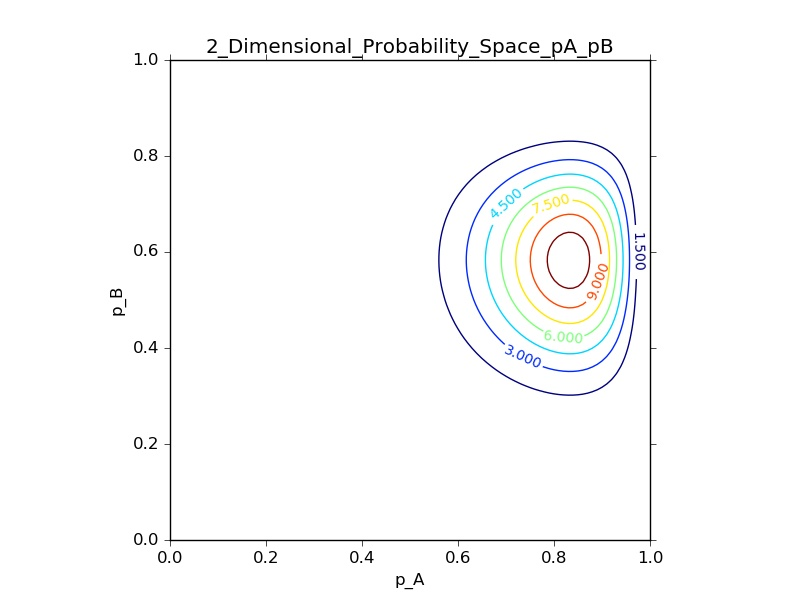
\includegraphics[width=90mm]{./figures/ab_stats_blog-1.jpg}
\caption{Contour Plot of the Likelihood of \((p_A, p_B)\) for \((n_A,
  m_A, n_B, m_B) = (12,10,12,7)\). The contours correspond to points
  of equal likelihood. The insides of high-value contour lines
  represent regions of high likelihood, with the peak at \((10/12,
  7/12)\). \label{fig:likelihood}}
\end{figure}
on which we've shown a contour plot of the likelihood function, see
the caption for additional explanation.

The implicit hypothesis that underlies most A/B experiments is that
``A is better than B''. For testing this hypothesis it is enough to
consider the {\em difference} between success probabilities
---i.e. \(p_A-p_B>0\)\footnote{See e.g. {\em A/B Testing}, Dan Siroker
  and Pete Koomen, Wiley (2013)}. (Before delving into the issue of
statistics, assume for a moment that we know both \(p_A\) and \(p_B\)
with certainty.) However, in most situations it is not enough
that A be simply better than B: Siroker and Koomen themselves include
an example of a test comparing a page with a static ad to one with a
video\footnote{{\em ibid.} ``Fail Fast and Learn'', pg. 79}. The
variant with the video was better in terms of both click-through and
conversion rates, but the costs of producing the video and displaying
it were deemed too high to launch the video version at scale. So while
the difference was statistically significant it wasn't {\em important}
enough from a business perspective. A complete approach requires the
analyst or business client to establish an {\em acceptance level} for
the metric \(M_{Acc}\) ---e.g. \(p_A-p_B>0.1\) for the difference
between A and B--- which would lead to a recommendation of A over
B. But now note that the analyst faces a choice of {\em metric} by
which to compare \(p_A\) and \(p_B\). E.g., in order to trigger
action, do we want the {\em difference} between success probabilities
to exceed \(0.1\) ---i.e. \(p_A-p_B>0.1\)--- or do we want the success
probability to {\em lift} by 20\% ---i.e. \(p_A > 1.2*p_B\)? There are
an immeasureable number of possible metrics and one has to determine a
metric that correlates linearly with business goals\footnote{To
  emphasize, note that the choice of comparison metric is an issue
  that arises {\em only} when we want to quantify the comparison. If
  we were only interested in {\em whether} Page \(A\) is better than
  Page \(B\), then any metric (as long as it is monotonic in \(p_A\)
  and \(p_B\)) would do. The choice of metric becomes important when
  we are interested not just in whether Page \(A\) is better than Page
  \(B\), but in addition, {\em by how much}.}.

We consider three metrics, discussed in Section~\ref{sec:metrics}. The
first two (the probability difference and lift mentioned above) are
very commonly used for Binary A/B testing but suffer some problems
which we point out at the end of Section~\ref{sec:metric_lift}. In
Section~\ref{sec:metric_odds_factor} we present the {\em odds factor},
which ---if the probability being measured is the {\em page transition
  probability}, that of moving to any other page on the website--- is
the average number of pages visited. Since number of page visits
correlates linearly to the number of conversion opportunities and
hence revenue, this is a good metric from a business perspective.

To get an idea of what the metrics look like and to compare them, in
Figure~\ref{fig:probmetrics} we plot the lines defined in
2-dimensional probability space \(\{(p_A,p_B)\}\) by a non-zero value
for each metric. If the line corresponds to a acceptable value for the
metric and the known success probabilities correspond to a point below
and to the right of the line, then \(A\) is deemed better than
\(B\). {\bf superimposed on pdf?}

Note that in reality we do not have a point \((p_A,p_B)\) that
corresponds to our knowledge of the success probabilities, instead we
have the likelihood \(f(p_A,p_B)\). Thus, we can ask for the {\em
  probability} that \((p_A,p_B)\) lies below the contour line for a
specific value, which is simply the volume of the likelihood
\(f(p_A,p_B)\) below the line, and is called the {\em credibility} of
the result. We show how to calculate this in
Section~\ref{sec:implementation}

Thus, we use the data to infer not just {\em which treatment is better}, but
in addition {\em by how much} and {\em how certain we are of
  this}. 

Since the inferences about ``better'' are probabilistic for any finite
data, the ``more better'' we want \(A\) to be ---i.e. the larger the
acceptable value for the difference--- the less credible it is that
\(A\) is better than \(B\) by that amount. In
Figure~\ref{fig:probmetrics}, the metric lines get squeezed
into the bottom right corner as the metric value increases. As a
one-dimensional example, if we obtained 60 Heads out of 100 trials, it
is much less likely to have arisen from a heavily loaded coin (say
\(p=0.80\)) than from a moderately loaded coin (\(p=0.65\)).

For concreteness, consider experimental data \((n_A, m_A) = (200,
40)\) and \((n_B, m_B) = (100, 15)\), and we will use the various
metrics to illustrate results. The analysis we've described so far
provides a {\em Metric vs. credibility} curve based on the
experimental data, of the form in Figure~\ref{fig:probdiff_vs_cred}
for the Probability Difference metric.
\begin{figure}[ht!]
\centering
% 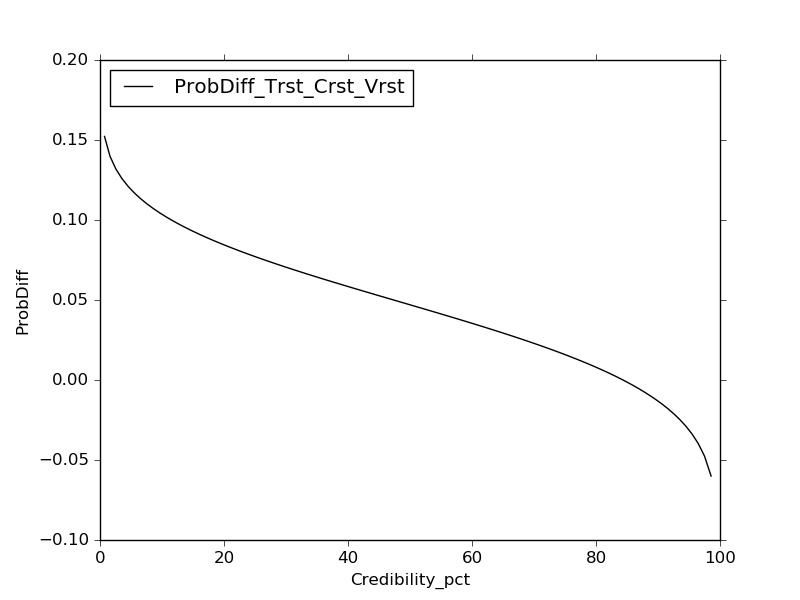
\includegraphics[width=90mm]{figures/ProbDiff_Trst_Crst_Vrst.jpeg}
\caption{Prob. Difference vs. Credibility \label{fig:probdiff_vs_cred}}
\end{figure}
The question then is how we can use this to make a recommendation
about \(A\) vs. \(B\). Recall that the business client has chosen a
comparison metric and a minimum acceptable value (say \(0.01\)) which
will lead to a recommendation for a business action. From the above
experimental curve, we or the client can certainly read off the
credibility at a given acceptance value to obtain a statement like
``\(0.02\) difference has \(70\%\) credibility'', but it is not yet
clear how to compare this or similar statements to the client's single
acceptance value. In our opinion, it is neither fair to place the onus
on the business client of defining a 2-dimensional acceptance point
``\(0.015\) difference at \(85\%\) credibility'', nor is it entirely
mathematically consistent (See Section~\ref{sec:memv}.).

How do we consistently compare the single value for acceptance
provided by the client to the credibility curves we've obtained? Note
that the client's threshold \(M_{Acc}\) is effectively the acceptable
value {\em at 100\% credibility}, or the acceptable {\em expected}
value, which we can now treat as a constant. On the other hand, from
the data, for each value (of a given metric), we obtain a credibility,
and we interpret the product of credibility and value as the {\em
  expected minimum value of the metric}. It is straightforward to show
that this expected minimum value has a maximum, as can be seen in
Figure~\ref{fig:exp_problift_vs_mvalue} where we've plotted the
Expected Minimum Value of the Probability Lift vs.~ the Probability
Lift itself.
\begin{figure}[ht!]
\centering
% 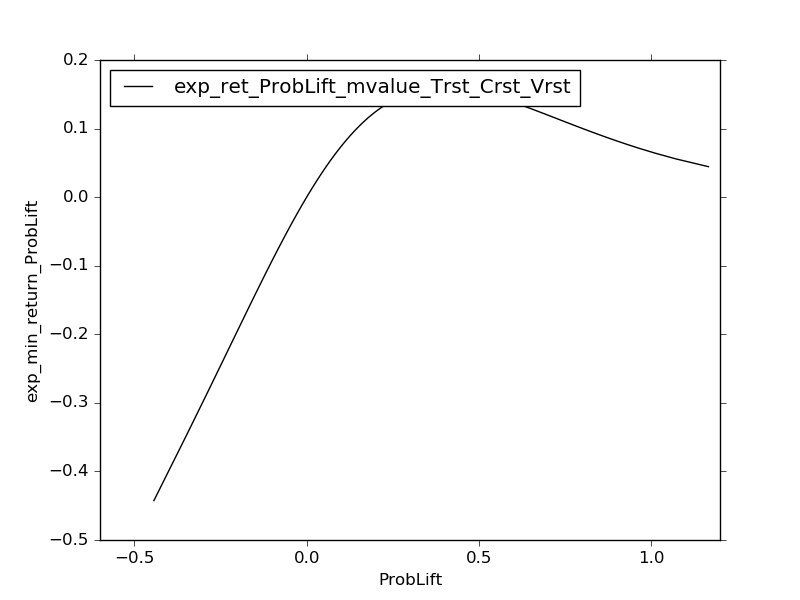
\includegraphics[width=90mm]{figures/exp_ret_ProbLift_mvalue_Trst_Crst_Vrst}
\caption{Expected Min(Lift) vs. Lift \label{fig:exp_problift_vs_mvalue}}
\end{figure}
The question is then reduced to comparing the experimentally
determined {\em maximum expected minimum value} to the client's
acceptable value: if the {\em max-min} is lower then the variant is
{\em not} better than the control.

In Section~\ref{sec:quantifying_comparison} we use the joint
likelihood to compute the credibility of any value of
one of the three comparison metrics. The credibility is calculated
numerically, by dividing the integration domain into small quantiles of
the likelihood (See Section~\ref{sec:implementation} for details.).

Finally, for the same sample data as in the example above, we describe
how to plot curves for the expected minimum value of the metric
vs. either the credibility or the metric value itself, for any of the
three metrics, e.g. Figure~\ref{fig:exp_oddsfactor_vs_cred}
Section~\ref{sec:results}. From these curves the maximum can be easily
read off and used to compare with the client's acceptable value and
provide the client with a yes/no answer.

\section{Summary of the Approach}

\subsection{The Data Model}\label{sec:data}
As a result of the experiment, for each test-variant pair, we obtain
\bi
\item \(n_A, m_A\) --- the number, respectively, of trials and
  successes on Page \(A\)
\item \(n_B, m_B\) --- the number, respectively, of trials and
  successes  on Page \(B\)
\ei

Table~\ref{table:1Dstats} summarizes some univariate descriptive
statistics for the sample results of each page, which we will compare
to those of the posterior distribution for the likelihood in
Section~\ref{sec:beta_props}
\begin{table}
\centering
\begin{tabular}{|l|l|} \hline \hline
Number of Trials & \(n\) \\ \hline
Number of Successes & \(m\) \\ \hline
Mean & \(\mu^F =\frac{m}{n}\) \\ \hline
Variance & \(\mu^F\cdot (1-\mu^F)\) \\ \hline
Variance of the Mean & \(\frac{\mu^F\cdot(1-\mu^F)}{n-1}\) \\ \hline
\hline
\end{tabular}
\caption{Descriptive Statistics of the Sample Results}
\label{table:1Dstats}
\end{table}

\subsection{Summary of the Approach}\label{sec:approach}
We approach the problem as follows:
\be
\item 
Given the input data (Section~\ref{sec:data}), calculate the Bayesian
posterior distribution (the likelihood) of \(p_A, p_B\) as in
Section~\ref{sec:bayesian2D}.
\item
Decide on a comparison metric \(M\) by which to {\em quantify the
  difference} between probabilities \(p_A\) and \(p_B\). See
Section~\ref{sec:metrics}.
\item 
Use the posterior distribution (computed in Step 1) to determine the
difference vs. credibility curve for a given comparison metric, see
Figure~\ref{fig:probdiff_vs_cred}
\item From the above, calculate the expected minimum metric
  vs. credibility curve and the maximum thereof (see
  Figure~\ref{fig:exp_problift_vs_mvalue}), which can be compared to
  the client's acceptance value.  \ee

\section{Bayesian Statistics}\label{sec:bayesian}

\subsection{Computing the Probability Distribution for One Population}
\label{sec:bayesian1D}
The probability of having \(m\) successes in \(n\) trials for a coin
that has an intrinsic probability of success \(x\) is given by the
Binomial distribution 
\beq
\label{eq:binomial}
P(m|x,n)={n \choose m}x^m (1-x)^{(n-m)}
\eeq
which is normalized over \(m\)
\beq
\label{eq:bin_normalized}
\sum_{m=0}^{n} P(m|x,n) = 1
\eeq

We wish to solve the reverse problem, namely, we wish to infer
(probabilistically) the intrinsic property of the coin given an
experimental outcome. For example, what is the likelihood that the
coin is fair when we obtained 7 Tails out of 10 trials? In other
words, given \(m, n\), derive \(f(x)\), the probability density
of \(x\).

We start by reminding the reader of Bayes' Theorem
\begin{equation}
\label{eq:bayes_theorem}
P(X|Y) = \frac{P(Y|X) \cdot P(X)}{P(Y)}
\end{equation}
In our context, this is re-written as follows
\begin{equation}
\label{eq:bayes_theorem_m_n}
f(x|n,m) = \frac{P(m|x,n)\cdot P(x)}{P(m)}
\end{equation}

Consider the three terms on the right hand side
\bd
\item  [\(P(x)\)] 
Given that we have no prior knowledge of the true probability,
\(P(x)\) is assumed to be the uniform distribution i.e., \(P(x)
=1\). 
\item [\(P(m|x, n)\)] This is the Binomial distribution
  Equation~\ref{eq:binomial}
\item [\(P(m)\)] This is ill-defined but drops out when we normalize
  the probabilities to integrate to 1.
\ed

With this normalization the distribution \(f(x|n,m)\) is the {\em Beta
distribution}
\footnote{\url{https://en.wikipedia.org/wiki/Beta_distribution}}
\begin{equation}
\label{eq:beta_for_m_n}
f(x|n,m) =\beta(x; m+1, n-m+1) = (n+1) {n\choose m}x^m (1-x)^{n-m}
\end{equation}

\subsection{Properties of the Beta Distribution}\label{sec:beta_props}
Some properties of the Beta distribution that are worth noting:
\bi
\item The domain of the Beta distribution is the unit interval  \(I =
  [0,1]\), and the Beta distribution is 0 at \(x=0,1\)  for all \(n,m
  >0\).
\item As we have stated before, the distribution is normalized over \(I\):
  \bdm
  \int_0^1 dx\cdot f(x|n,m) = 1
  \edm
\item In the case where we have {\em no} data, i.e. \(n=m=0\), the
  posterior distribution is the uniform distribution
  \bdm
  f(x|0,0)=\beta(x|1,1) =1
  \edm
\item The mode, or the value of \(x\) at which the distribution is a
  maximum, is given by
  \bdm
  {\tt mode}(x) = {\tt argmax}(\beta(x|m+1, n-m+1)) = \frac{m}{n}
  \edm
  which is the experimental mean. Thus the experimental mean
  predicts the maximum likelihood.
\item From the properties of the Beta distribution,
the mean of the Bayesian distribution,
\begin{equation}
\label{eq:beta_mean}
\mu = \int_0^1 dx \cdot x\cdot f(x|n,m) = \frac{m+1}{n+2}
\end{equation}
Note first that this is {\em not} equal to the mode, in fact the mean
regresses from the mode towards 0.5, which, in the absence of other
information is the mean probability of the outcome of a binary valued
experiment.  Note also the difference between
\(\mu^{Bayes}=\frac{m+1}{n+2}\) in Equation~\ref{eq:beta_mean} and the
mean of the experimental distribution \(\mu^F=\frac{m}{n}\) in
Table~\ref{table:1Dstats}. This is because the Beta distribution adds
2 ``pseudo-trials'', one being a success and the other being a
failure, to the observed trials. This is consistent with the Bayesian
prior probability distribution \(P(x) = 1\).
\item The Beta distribution is not symmetric about the mean,
  except for the special case \(a=b\), in which case \(\mu = 0.5\):
  \begin{equation}
  \label{eq:beta_symmetric}
  \beta(x|a,b) = \beta(2 \cdot \mu-x|a,b) \iff a=b
  \end{equation}
\item The variance of the distribution is 
  \begin{equation}
  \label{eq:beta_variance}
  \sigma^2 = \frac{\mu\cdot(1-\mu)}{n+3}
  \end{equation}
  which is different from the variance of the mean in
  Table~\ref{table:1Dstats} in two ways: the mean here is that of the
  posterior distribution, not the Frequentist mean as in the table,
  and the denominator includes the two extra ``psuedo-trials''.

\begin{comment}
\item Since we've calculated the mean and the variance, we can
  approximate the Beta distribution by a normal distribution with
  the mean (Equation~\ref{eq:beta_mean}) and variance
  (Equation~\ref{eq:beta_variance}),
  {\it not} the mean and variance in Table~\ref{table:1Dstats}. In doing this
  approximation, one must be aware of the following differences
  \be
  \item the normal distribution has support outside the unit interval, 
  \item is finite at the bounds of the interval and 
  \item is symmetric about the mean, 
  \ee
\end{comment}

\item Finally, the Beta distribution satisfies an obvious
  multiplication law, which we've expressed in terms of \(f(x)\)
  \beq\label{eq:beta_multiplication} f(x|m,n)\cdot f(x|m_0,n_0)
  \propto f(x|n+n_0, m+m_0)
  \eeq
  The implication of this is that the results of consecutive
  experiments are additive: Consider a situation in which the trial
  period of an experiment yields results \((n_0,m_0)\) and the
  subsequent experiment yields \((n,m)\). For consistency's sake, we
  require that the Bayesian posterior probability be determined by the
  cumulative results \((n+n_0, m+m_0)\). We see that this is true: the
  {\em prior} probability distribution \(P(x)\) in
  Equation~\ref{eq:bayes_theorem_m_n} arises as the posterior to results
  \((n_0, m_0)\). Then \(P(x) = f(x|n_0, m_0)\). Hence the probability
  distribution posterior to the subsequent experiment with results
  \((n,m)\) is given by \(P(m|x,n)\cdot f(x|n_0,m_0)\). The
  multiplication rule above, Equation~\ref{eq:beta_multiplication}
  then implies that the consistency condition is satisfied.
\ei

\subsection{Computing the Joint Probability Distribution for the Two Populations}\label{sec:bayesian2D}
Now that we have the individual PDFs for \(A,B\)
\begin{equation}
\label{eq:fa_fb}
\begin{split}
f_A(x)=f(x|n_A,m_A) = \beta(x|m_A+1, n_A-m_A+1) \\
f_B(y)=f(y|n_B,m_B) = \beta(y|m_B+1, n_B-m_B+1) \\
\end{split}
\end{equation}
we can 
compute the joint probability density \(f(x, y) = P[p_A=x, p_B=y]\) 
\begin{equation}
\label{eqn_joint_pdf}
f(x,y) = f_A(x)\cdot f_B(y)
\end{equation}
where we use the fact that user behavior on page \(A\) is independent
of user behavior on page \(B\).

We now have the posterior probability refered to in Step 1 of
Section~\ref{sec:approach}

\section{Comparison Metrics}
\label{sec:metrics}
In this section, we elaborate on the metrics summarized in
Table~\ref{table:metrics}
\begin{table}
\centering
\begin{tabular}{|l|r|c|l|l|} \hline \hline
{\bf Metric} & {\bf Section} & {\bf Parameter} & \(\bb{M(x, y) > 0}\) & {\bf Boundary: }\(\bb{y = m(x)}\) \\ \hline \hline
Difference & \ref{sec:metric_diff} & \(\delta\) & \(x - y - \delta\)& \(y = x - \delta\) \\ \hline 
%
Lift & \ref{sec:metric_lift}& \(\lambda\) & \(x - y \cdot (1+\lambda)\) & \(y = \frac{x}{1+\lambda}\)\\ \hline 
%
Odds Factor & \ref{sec:metric_odds_factor} & \(\phi \)
& \(O(x)-\phi\cdot O(y)\)
  & \(y = O^{-1} \left( \frac{O(x)}{\phi}\right)\)\\ \hline
\hline
\end{tabular}
\caption{Summary of Metrics}
\label{table:metrics}
\end{table}

\subsection{Probability Difference}
\label{sec:metric_diff}

The intuition here is that we consider \(A\) to be better than \(B\)
if the intrinsic probability \(p_A\) exceeds \(p_B\) by some constant
\(\delta\). This metric has many drawbacks, but to illustrate one,
consider rows 1 and 2 in Table~\ref{table:examples}:
\begin{table}
\centering
\begin{tabular}{|l|r|r|r|r|r|r|r|r|} \hline\hline
  {\bf Row} & \(\bb{n}\) & \(\bb{m_B}\) & \(\bb{m_A}\) & \(\bb{y}\) & \(\bb{x}\) & Diff. \(\delta\) & Lift \(\lambda\) & Odds F.\(\phi\) \\
  \hline\hline
  1 & & & & \(0.50\) & \(0.55\) & \(0.05\) & \(10\%\) & \(1.2\)\\ \hline
  2 & & & & \(0.05\) & \(0.10\) & \(0.05\) & \(100\%\) & \(2.1\)\\ \hline
  3 & & & & \(0.04\) & \(0.10\) & \(0.06\) & \(150\%\) & \(2.7\)\\ \hline 
  4 & \(10k\) & \(9\) & \(10\) & \(0.9m\) & \(1.0m\) & \(0.1m\) & \(11.1\%\) & \(1.11\)\\ \hline
  5 & \(10k\) & \(9-1*\sigma=6\) & \(10\) & \(0.6m\) & \(1.0m\) & \(0.4m\) & \(67\%\) & \(1.67\)\\ \hline
  6 & & & & \(0.90\) & \(0.95\) & \(0.05\) & \(5.6\%\) & \(2.1\)\\
  \hline\hline
\end{tabular}
\caption{Metrics: Examples}
\label{table:examples}
\end{table}
An increase in Row 1 from \(0.50\) to \(0.55\) feels intuitively very
different from the increase in Row 2 from \(0.05\) to \(0.10\), yet
the difference in both cases is the same \(0.05\).

\subsection{Probability Lift}
\label{sec:metric_lift}
We could address the above drawback of the difference metric
(Section~\ref{sec:metric_diff}) by measuring the 
increase in terms {\em relative} to Control. For example, one could
want the Variant to result in 10\% greater conversion ratio than the
Control. The desired {\em lift} is often written as
\begin{equation}
\label{eq:lift}
\lambda = \frac{x-y}{y}
\end{equation}

In Rows 1 and 2 in Table~\ref{table:examples}, the lift changes from
10\% to 100\% and captures our intuition about the ``bigness'' of the
change. One problem with this metric is that often, a large lift is
nothing more than a measure of the smallness of the effect in the
Control group, and exposes the decision to the vagaries of an
ill-chosen control group. A related problem with this metric is that
it is {\em non-linearly} sensitive to errors in the Control
\(y\). Consider the small drop in \(y\) from \(0.05\) to \(0.04\)
between Rows 2 and 3, which causes a dramatic increase in the lift
from 100\% to 150\%.

Such errors can easily arise due to poor statistics, even with a large
number of trials. In Row 4, there were only 9 successes in the control
group. The standard error in the number of successes is \(\sqrt{9}
=3\), which translates into a (conservatively underestimated) 15\%
probability of getting 6 or fewer successes (Row 5). So without any
likely {\em real} change in the property of the population, this
``noise'' causes the lift to jump by a factor of \(6\) from \(11\%\)
to \(67\%\), even though \(y\) has only decreased by a third!

Finally, neither of these two metrics captures the fact that it is
just as important to reduce the failures as it is to increase the
successes. Consider the difference between Rows 2 and 6:
\be
\item In Row 2 an increase in probability from 0.05 to 0.10
  corresponds to a lift of 100\%
\item In Row 6 an increase in probability from 0.90 to 0.95
  corresponds to a lift of only 5.6\%
\ee
On the other hand, the jump from 0.90 to 0.95 in Row 6 means that we
have done 50\% as well as we could have, given that we could not go
higher than 1.  The jump from 0.05 to 0.10 in Row 2 means we did only
5.6\% as well as we could have. Is there a metric that captures how
much better we've done in comparison to how much better we {\em could
  have} done?

Consider also the following flaw with the above two metrics: From a
methodological or product design standpoint, one should establish the
acceptance value for the metric that triggers a business action {\em
  before} starting the experiment: first, so as to not get vested in
the positive outcome of an experiment and second, because the business
environment under which decisions are being made is mostly the same
before and after the experiment. From this standpoint, both the
difference and lift metrics fail. A reasonable acceptance value cannot
be established {\em before} knowing what the control results are. For
example, while a pre-established minimum lift of 100\% is entirely
reasonable if it turns out the control group's success rate is 0.05, a
lift of 100\% is absurd if the control group's success rate turns out
to be 0.9.

For important but more abstract mathematical problems with the above
two metrics, see the expanded version of this article.

\subsection{Odds Factor and Related Metrics}
\label{sec:metric_odds_factor}
A common measure of traffic to a website is the number \(P\) of page
visits per session. This metric is useful since it is reasonable to
assume that on average page visits is proportional to viewing
opportunities to click or convert which in turn is linear in revenue.
Suppose that the probability \(p\) that we've measured is the {\em
  page transition probability} for the website, the probability that
the user visits another page on the website as opposed to leaving the
website, timing out or otherwise ending the session. Straightforward
algebra shows that the average number of page visits per user-session
is given by
\beq
P = p+ p^2 + p^3 ... = \frac{p}{1-p}
\eeq
This is nothing but the {\em odds ratio} or simply the odds
corresponding to the probability. It overcomes the problems with the
probability difference and the lift discussed above, and in addition,
is both mathematically sound and familiar to non-technical people.
\begin{definition}
\label{def:odds}
For a probability \(p\), the odds \(O(p) = \frac{p}{1-p}\)
\end{definition}

From the odds \(o\), the probability can be recovered by
\beq
\label{eq:podds}
O^{-1}(o) = \frac{o}{1+o}
\eeq

This is a metric familiar to gamblers. Why do gamblers think in terms
of odds rather than probabilities? In a {\em pay-to-play} situation
they intuitively understand that when evaluating a position they have
to take into account the cost of failure \$\(C\) as well as the
benefits of success \$\(B\). They are evaluating and optimizing the
{\it benefit-to-cost-ratio}
\bdm
\frac{\$B \cdot p}{\$C \cdot (1-p)}
\edm
Since both \$\(B\) and \$\(C\) are presumed independent of \(p\), these
drop out of consideration and one wants to increase the odds.  So to
compare the results of \(A\) and \(B\) one metric we will look
at is
\beq
\label{eq:oddsfactor}
O(x) > \phi\cdot O(y)
\eeq
This is interpreted as saying that the odds associated with \(A\) are
at least \(\phi \times\) the odds associated with \(B\). We will
consider minor modifications of this metric, such as the page views
difference and the page views lift, in a future article.

Note in Table~\ref{table:examples} that the odds factor is much more
stable w.r.t. errors in \(y\), in the sense that it behaves
linearly. For example, between Rows 4 and 5 the control probability
drops by a third, and the odds lift increases \(1.5\times\), as
opposed to the \(6\times\) increase in the lift.

\subsection{Comparison of the Metrics}
\label{metric_comparison}
In order to get a better feeling for the metrics, for each of them,
Figure~\ref{fig:probmetrics} shows their contours in 2D probability space for
the comparison parameter values in Table~\ref{table:param_values}.
\begin{table}
\centering
\begin{tabular}{|l|l|l|r|} \hline \hline
{\bf Metric} & {\bf Section} & {\bf Comparison Parameter} & {\bf Value}  \\ \hline \hline
Difference & \ref{sec:metric_diff} & \(\delta\) & 0.25 \\ \hline 
%
Lift & \ref{sec:metric_lift}& \(\lambda\) & 1.0\\ \hline 
%
Odds Factor & \ref{sec:metric_odds_factor} & \(\phi \)
& 2.0\\ \hline
\hline
\end{tabular}
\caption{Values of Comparison Parameters for Fig.~\ref{fig:probmetrics}}
\label{table:param_values}
\end{table}
We note that the ranges of both the difference metric and the lift are 
bounded and do not apply to all values of \((x,y)\). The odds factor has no
such limitations.

\begin{figure}[ht!]
\centering
% 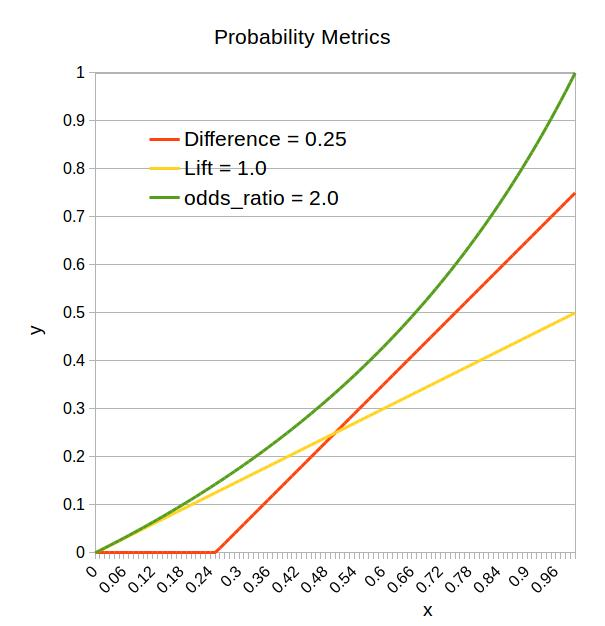
\includegraphics[width=90mm]{figures/probability_metrics}
\caption{Probability Comparison Metrics on 2D Probability
  space \label{fig:probmetrics}}
\end{figure}

There are a few other things to note. When their threshold values are
0, the boundaries for all metrics collapse to the \(45^\circ\)
diagonal line, and all the Bayesian credibilities will be the same.
However, when the thresholds have non-zero values, the boundaries are
{\em not} the same. As we can see in Fig.\ref{fig:probmetrics}, there
can be large gaps between the different metric lines at all values of
\(x\). When the likelihood has signficiant support in either of those
regions, the metrics will lead to contradictory decisions. {\bf seems
  to call for a superimposed plot of pdf and metric contours?}

\section{Comparing Pages \(A\) and \(B\) quantitatively}
\label{sec:quantifying_comparison}
In order to quantify the comparison of Page \(A\) and Page \(B\), we
choose one of the metrics \(M(x, y)\) from Table~\ref{table:metrics}
discussed in Section~\ref{sec:metrics} above. The metric may have a
non-zero threshold as an argument.  \(M\) is a mapping from the unit
square \([0,1] \times [0, 1]\) into \(\cal{R}\).  Given a comparison
metric \(M\), the {\em credibility} that \(M>0\) or the probability
that Page \(A\) is better {\em in terms of metric} \(M\) than Page
\(B\) is
\begin{equation}
\label{eq:vol_under_surface}
{\tt Credibility}[M>0]=\int_{M(x,y) >0} f(x, y)\,  dy \, dx
\end{equation}

Most reasonable choices for \(M\) are such that we can rewrite
Equation~\ref{eq:vol_under_surface} as 
\begin{equation}
\label{eq:vol2}
\int_{x=0}^{x=1} f_A(x) \left( \int_{y=0}^{y=m(x)} f_B(y)\,  dy\right) dx
\end{equation}
where \(m(x)\) is
the solution, for \(y\), of \(M(x, y) = 0\). (See the last column of
Table~\ref{table:metrics}.)

We will evaluate the double integral in 2 steps.  In the first step,
we note that the term within the parentheses has a closed form
solution \(\beta_{cf}(m(x); m_B+1, n_B-m_B+1)\), where \(\beta_{cf}\)
is the cumulative function of the Beta distribution. This allows
us to rewrite Equation~\ref{eq:vol2} as
\begin{equation}
  \label{eq:vol3}
  \begin{split}
    {\tt Credibility} &= \\
    &\int_0^1dx\cdot \beta(x,m_A+1, n_A-m_A+1) \beta_{cf}(m(x), m_B+1, n_B-m_B+1)
  \end{split}
\end{equation}
which is then evaluated numerically.

\subsection{Implementation Detail: Integrating the Product of the Beta Distributions}\label{sec:implementation}
The Python package {\tt scipy.stats} includes the \(\beta\) distribution
{\tt beta.pdf(p|a,b)} and its cumulative function {\tt beta.cdf(p|a,b)}
  \begin{equation}
  \label{eq:beta_cf}
  \beta_{cf}(x|a,b) = \int_0^{x'}dx'\cdot\beta(x'|a,b)
  \end{equation}

For numerical plotting routines or for numerical integration one
discretizes the domain \(x\) into a set of points at which to evaluate
the beta distribution or its cumulative function.  For any number of
points which break up the domain into uniform intervals, and for any
given tolerance for error, there exists a number of trials \(n\) which
is large enough that the effective support of the Beta distribution is
smaller than an interval, resulting in graphical or numerical
integration errors which exceed the tolerance. The graph will be
either flat or contain an arbitrary valued spike and the integral will
jump from \(0\) to some absurdly large value.

So what can we do? Very usefully, the quantile function or the inverse
of the cumulative function {\tt beta.ppf(percentile|a,b)} ---which
allows one to calculate the values of \(p\) at which a given
percentile of the distribution occurs--- is also implemented as a part
of {\tt scipy.stats}. Intuitively, what we want to do is to integrate
or plot over a subset of the domain with some large proportion of the
support. Assuming that we can tolerate an error of ~0.2\%, we choose a
subset with 99.8\% of the support. Then we can use {\tt beta.ppf} to
calculate the minimum and maximum values of the discrete set as
\beq
\begin{split}
  x_{0.1\%}&={\tt beta.ppf(0.001|m+1, n-m+1)}\\
  x_{99.9\%}&={\tt beta.ppf(0.999|m+1, n-m+1)}  
\end{split}
\eeq

One is again tempted to break up the subset
\([x_{0.1\%},x_{99.9\%}]\) into uniform intervals, but in fact the thing
to do is to break it up so that the intervals are smaller where the
distribution is larger and vice versa. This corresponds to finding the
\(x-\)values for {\em uniformly distributed quantiles} ---we are
effectively discretizing the {\em range} of the cumulative function
uniformly, {\em not} the domain of the PDF:
\bdm
{\tt Array(x)} = {\tt beta.ppf(Array([0.001, 0.999, step = 0.001])|m+1, n-m+1)}
\edm
Since ``(99.8\% of) everything'' is happening in this range of
\(x\) values, using this array for numerical integration limits the errors.

\subsection{Choosing an array of metric values}
Due to considerations similar to the ones discussed above for
integrating the probability distribution, one needs a ``dynamic'' way
of determining a ``good'' range of metric values at which to evaluate
the credibilities. Most low or high values of the metric will have
credibilities of 1 or 0 respectively\footnote{For example, when the
  metric value is small and such that the metric line is to the left and above
  the support of the probability distribution, the credibility or
  volume under the curve will be 1.}, and will vary between those
extremes only for values of the metric where the metric line crosses the
support of the probability distribution. No matter how fine-grained
the static metric array is, there will be some narrow probability
distribution which causes the credibility to abruptly jump from 0 to
1. Our approach to solving this is as follows:
\be
\item Calculate the mean and variance of the Bayesian distribution for the probabilities \(x=p_A, y=p_B\).
\item Calculate approximations to the mean and the variance of the metric \(M(x,y)\) using the results derived in {\tt mean\_and\_variance\_of\_function.pdf}.
\item Use these values in a normal approximation to the distribution of the metric to calculate the array of metric values corresponding to the percentiles
  \beq
  \begin{split}
    {\tt Array(min(M))} = &{\tt norm.ppf(Array([0.01, 0.99, step = 0.01])}\\
      &{\tt |loc = mean, scale = sqrt(var))}
    \end{split}
\eeq
\ee

\subsection{Maximum Expected Minimum Value}\label{sec:memv}
For each value of \(M\) in the array constructed above, we can use
Equation~\ref{eq:vol3} to calculate the credibility
\beq\label{eq:credarray}
{\tt Array}(Cred) = {\tt credibility(Array}(min(M)))
\eeq
These arrays can be used to plot the metric vs. credibility
curves. Note that this is the credibility of the minimum value of the
comparison metric, i.e. the probability that the actual value of the
metric is larger than this minimum. Is this not sufficient to compare
to the client's acceptance value \(M_{Acc}\)? Recall that \(M_{Acc}\)
is implicitly the value that the client will accept (for the test to
trigger a recommendation for A over B) at \(100\%\) credibility. From
the perspective of the expected outcome, this is equivalent to their
accepting a higher metric value at lower credibility,
e.g. \(1.11*M_{Acc}\) at only \(90\%\) credibility since the
expectation values are the same \(M_{Acc}*1.0 = 1.11*M_{Acc}*
0.90\). So the client's expected acceptance value defines a curve in
metric vs. credibility space
\beq\label{eq:expacc}
M*Cred(M)=M_{Acc}
\eeq
This curve is a hyperbola and does {\em not} belong to the family of
(inverse) sigmoidal curves as do the metric vs. credibility curves,
e.g. Figure~\ref{fig:probdiff_vs_cred}. In general, the client
acceptance curve will intersect the metric vs. credibility curve in 0
or 2 points\footnote{Ignoring the pathological situation where they are
tangent.}.

Consider the situation where the client has been asked to provide a
2-dimensional decision point \((Cred_{Acc},M_{Acc})\). This defines an
acceptance curve of points which are equivalent to each other from an
expected value perspective:
\beq
M*Cred(M)=M_{Acc}*Cred_{Acc}
\eeq
If there are no intersections the recommendation is unambiguous, A is
not better than B. However, if there are two intersections, the
recommendation is ambiguous since it implies that there are points on
the acceptance curve below the metric vs. credibility curve that
trigger a ``Yes'' recommendation but that there are equivalent points on the
acceptance curve that are above the metric vs. credibility curve that
do not trigger a recommendation. This is the ambiguity in the
two-dimensional decision point approach we referred to earlier.

So we require from the client a single expected acceptance value
\(M_{Acc}\) which defines a curve Equation~\ref{eq:expacc}. From the
credibility array Equation~\ref{eq:credarray} we can construct the
array of expected minimum metric values since
\bdm
Expected(min(M)) = Cred(M)*min(M)
\edm
One can show that the \(Expected(min(M))\) has a maximum which we
denote by \({\tt MaxExpMin}(M)\). This can be found from the above
array and can be visualized e.g. in
Figure~\ref{fig:exp_problift_vs_mvalue} where the \(Expected(min(M))\)
of the probability Lift has been plotted against the va;lue of the
lift itself. To make a recommendation, we proceed as follows.

\subsection{Recommendation}
The maximum expected minimum value determined above from the data is
compared to the {\em Acceptance} value \(M_{Acc}\) for the metric \(M\)
established by the business client:
\begin{definition}
If \({\tt MaxExpMin}(M) \leq M_{Acc}\quad{\rm then}\quad A\quad{\rm
  is\quad not\quad better\quad than\quad}B\)
\end{definition}
Like most scientific tests, strictly speaking it is only good for
ruling out the null hypothesis. However, we can recommend
\begin{definition}
If \({\tt MaxExpMin}(M) > M_{Acc}\quad{\rm then}\quad A\quad{\rm
  is\quad better\quad than\quad}B\)
\end{definition}

\section{Sample results for Bayesian Credibility}
\label{sec:results}
For test results with \((n_A, m_A, n_B, m_B) = (200, 40, 100, 15)\), we plot
the credibility as a function of the importance levels for the three metrics
proposed above. {\bf show all three curves for one metric only as example?}

\subsection{Probability Difference}
From Figure\ref{fig:probdiff_vs_cred} the user can read-off the
probability difference that corresponds to a chosen credibility, or
vice versa. We see that as expected the credibility drops as the
difference between \(p_A\) and \(p_B\) increases. As described in the
Introduction Section~\ref{sec:intro}, the business client or analyst
can compare the position of the metric-credibility curve in the figure
to the decision point (threshold metric, credibility) and decide
whether to proceed with the business action.

\subsection{Probability Lift}
From Figure~\ref{fig:exp_problift_vs_mvalue} the user can read-off the
maximum expected minimum lift which can be compared to \(Lift_{Acc}\).

\subsection{Odds Factor}
\label{sec:odds-factor-result}
\begin{figure}[ht!]
\centering
% 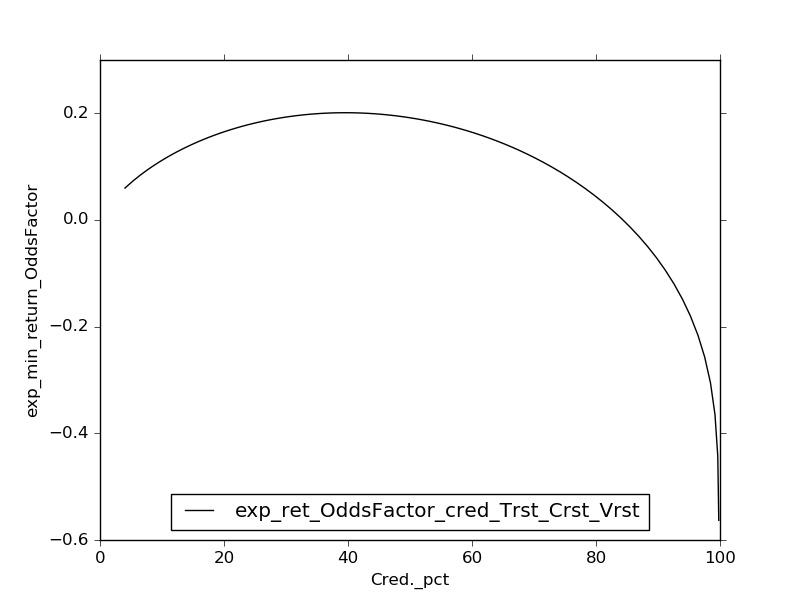
\includegraphics[width=90mm]{figures/exp_ret_OddsFactor_cred_Trst_Crst_Vrst}
\caption{Expected Min(Odds Factor) vs. Credibility
  \label{fig:exp_oddsfactor_vs_cred}}
\end{figure}
From Figure~\ref{fig:exp_oddsfactor_vs_cred} the user can read-off the
maximum expected minimum odds factor\footnote{As an aside, we point
  out that, due to the symmetries of the odds and those of the Beta
  distribution, the Odds Factor vs. credibility curve is invariant
  under the discrete symmetry
\bdm
(n_A, m_A, n_B, m_B) = (n_B, n_B - m_B, n_A, n_A - m_A)
\edm.}.

\section{Conclusion}

For both the test and control populations of a binary outcome A/B test
the number of trials and successes are counted. We've taken the
Bayesian approach to calculate the posterior joint likelihood for the intrinsic success probabilities of the two
populations from the experimental data. Separately, and possibly
before the experiment is started, based on the business outcome
desired a comparison metric is chosen, and an {\em acceptance value}
\(M_{Acc}\) which will trigger a recommendation. For the chosen metric, a metric
vs. credibility curve is calculated from the joint probability
distribution, and from this in turn a plot of the expected minimum
metric vs. the credibility. The maximum of this is found, the {\tt
  MaxExpMin}(M). A business action is recommended based on comparing
{\tt MaxExpMin}(M) to \(M_{Acc}\).

\section{Appendix}\label{sec:app_frequentist}
In this section we will briefly outline the Frequentist approach and
then compare it to the Bayesian approach we have taken in this paper.

\subsection{The Standard Frequentist Approach}\label{sec:frequentist}
The material in this section is well-known and is included for completeness
and comparison. For an utterly convincing argument that demonstrates the
superiority of the Bayesian approach without assuming any {\em a priori}
knowledge of statistics, please take the time to read
\url{https://xkcd.com/1132/}.

\subsubsection{Single Variant}\label{sec:frequentist1D}
Consider the situation for one variant as described earlier in Section
\ref{sec:bayesian1D}, with \(n\) trials indexed by \(i\) and the corresponding
outcomes \(x_i\in \{0,1\}\). Let there be \(m\) successes (\(1\))
and \(n-m\) failures (\(0\)). Then the mean or expectation of \(\{x_i\}\) is
\bdm
\mymean{x} = \mu = \frac{1}{n}\sum_i x_i = \frac{m}{n}
\edm
and the variance of the distribution is
\bdm
var(x) = \sigma^2_x = \mu\cdot(1-\mu)
\edm
where \(\sigma_x\) is the standard deviation.

Now, we are primarily interested in the variance or the Standard Error
in the estimated mean. From the definition of variance, it is fairly
easy to show that the variance of the mean is
\bdm
var(\mu) = \sigma_F^2 = var(\mymean{x}) = \frac{var(x)}{n} =
\frac{\mu\cdot(1-\mu)}{n}
\edm
One then uses
the above parameters to calculate the \(z\)-score corresponding to
some proposition about \(\mu\), assumes that \(\mu\) is normally
distributed and uses the cumulative function of the Normal
distribution to calculate the percentiles or \(p\)-value from the
\(z\)-score.

\subsubsection{The confidence that A is better than B}
Suppose we were interested in the proposition that \(M(x,y, \delta)
>0\), where \(x,y\) are the probabilities associated with variants A
and B respectively and \(M(x,y)\) is one of the comparison metrics
defined earlier with minimum acceptable value \(\delta\). If we had
estimates for \mymean{M} and \(SE(M)=\sqrt{var(M)}\) then we could
calculate the \(z\)-statistic for the proposition via
\beq\label{eq:zstat}
z(M)= \frac{\mymean{M}}{SE(M)}
\eeq
and proceed to calculate the parametric confidence level or \(p\)-value.
Since we are only interested in whether A is better than B, the
(1-sided) proposition we want to test is whether the probability
associated with variant A is greater than the probability associated
with variant B, i.e., \(M(x,y) = x - y >0\). The proposition is
\beq
M(x,y) = x-y> 0
\eeq
from which
\beq
\begin{split}
  \mymean{M} &=\mymean{x} - \mymean{y}\\
  var(\mymean{M}) &= var(\mymean{x})+var(\mymean{y})\\
  z(x>y) &= \frac{\mymean{x} - \mymean{y}}{var(\mymean{x})+var(\mymean{y})}
\end{split}
\eeq

\subsection{Reasons to Prefer Bayesian to Frequentist}\label{sec:bayes_over_freq}
Our reasons to prefer the Bayesian approach to the Frequentist are listed below:
\be
\item The Frequentist approach involves a parametric approximation
  usually based on the normal distribution, which is not defined on
  probability space and is notoriously inaccurate for situations with
  low numbers of trials as well as those with probabilities near 0 or
  1.

  The Bayesian approach doesn't assume normality, it derives the
  form of the posterior distribution.
\item In the Frequentist approach, the results of the parameteric
  calculations depend on the the metric used for comparing the two
  probabilities \(p_A\) and \(p_B\). In the first place normality is
  not preserved under nonlinear transformations, e.g. if \(x\) is
  normally distributed, \(e^x\) is not. In the second place, the
  calculation of the descriptive statistics for non-linear metrics is
  somewhat non-trivial and involves an approximation\footnote{See {\tt
      mean\_variance\_of\_function.pdf}.}. Furthermore, the actual
  values of the confidence levels depend on the algebraic form of the
  metric. For example,
  \beq
  \begin{split}
    &P[\frac{1-y}{1-x} - (1-\lambda_0)>0]\quad{\rm and}\\
    &P[(1+\lambda_0)\cdot x -y-\lambda_0>0]
  \end{split}
  \eeq
  are the probabilities of logically equivalent propositions but
  the outlined approximations to calculating them lead to different
  values of the confidence.

  The Bayesian approach (at least in the case of the Binary tests
  considered here, for which the posterior distributions can be
  constructed and the required integrations carried out numerically)
  can be applied to any comparison metric on 2D probability space, is
  well-defined and does not need to be approximated.
  \item The Frequentist/parametric approach breaks down when either
    trials or successes are small in number and one has to take care
    with the use of the standard errors.

    When the numbers are small, the Bayesian distribution has a large
    variance that reflects our uncertainty in the intrinsic
    probability and it can be applied without treating the small
    number situation as a special case.
    \ee

For a discussion of the above reasons, for details on calculating the
Frequentist confidence levels for the different metrics described here
in Section~\ref{sec:metrics} and for limits on the domain of validity
for which Frequentist calculations approximate the Bayesian ones, see
{\tt frequentist\_vs\_bayesian.pdf}.

\end{document}


\footnote{We leave a discussion of cost based metrics
  (e.g. donation amount per page visit) and some theoretical binary metrics
  to future articles.}  
